\chapter{Malware difundido en redes sociales}

\begin{tcolorbox}[
    title=Detalles de la Noticia, 
    colframe=black, % Borde negro
    colback=gray!5,         % Fondo gris claro
    sharp corners,          % Esquinas afiladas
    breakable              % Permite que el cuadro se divida en varias páginas
]

    % 1. Descripción y Título
    \textbf{Breve descripción de la amenaza: (más de 100 palabras)}
    \vspace{0.5em}
    La amenaza central descrita es el uso de malware de tipo \textit{infostealer} 
    (ladrones de información), específicamente familias detectadas en la "Operación Secure" 
    como Lumma, RisePro, Meta Stealer, Vidar y Rhadamanthys. Estos programas maliciosos están diseñados con el objetivo principal de infiltrarse en dispositivos de víctimas para extraer de forma silenciosa datos extremadamente sensibles. Entre la información comprometida se encuentran credenciales de acceso almacenadas en navegadores, cookies de sesión (que permiten saltarse la autenticación de doble factor), datos de carteras de criptomonedas y detalles financieros. El vector de ataque mencionado incluye técnicas de ingeniería social, campañas de phishing y fraudes en aplicaciones de citas o redes sociales. Una vez que el malware infecta el sistema, recopila la información y la envía a servidores de comando y control (C2). Los datos robados suelen ser vendidos en foros clandestinos de la Dark Web o utilizados directamente por los atacantes para realizar fraudes bancarios, suplantación de identidad o facilitar ataques de ransomware a mayor escala contra infraestructuras corporativas.
    \vspace{0.5em}

    \textbf{Fecha de la noticia:}
    \vspace{0.5em}
    14 de junio de 2025

    \textbf{Título de la noticia:}
    \vspace{0.5em}
    \href{https://www.escudodigital.com/ciberseguridad/operacion-secure-infostealer.html}{Interpol desmantela red global de malware infostealer con 32 detenidos}

    % 2. Enlaces y Medio
    \textbf{Enlace a la noticia:}
    \vspace{0.5em}
    \href{https://www.escudodigital.com/ciberseguridad/operacion-secure-infostealer.html}{https://www.escudodigital.com/ciberseguridad/operacion-secure-infostealer.html}

    \textbf{Medio:}
    \vspace{0.5em}
    Escudo Digital
    
    \textbf{Enlace al medio:}
    \vspace{0.5em}
    \href{https://www.escudodigital.com/}{https://www.escudodigital.com/}

    \textbf{Nacionalidad del medio:}
    \vspace{0.5em}
    España
    
    \textbf{Idioma de la noticia:}
    \vspace{0.5em}
    Español
    
    \textbf{Pequeña imagen de la noticia:}
    \newline
    \vspace{1em}
    \begin{center}
        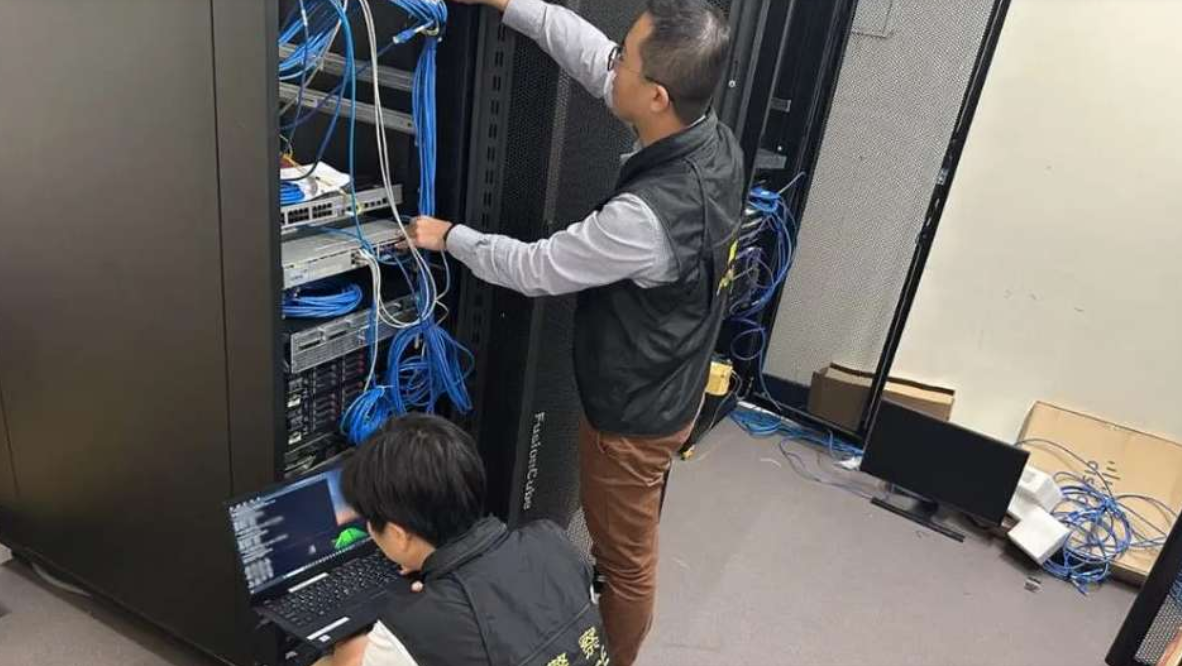
\includegraphics[width=0.8\textwidth]{Imagenes/03-mal.png} 
    \end{center} 

    % 4. Resumen y Análisis
    \textbf{Breve resumen de la noticia: (más de 100 palabras)}
    \vspace{0.5em}
    Interpol ha liderado una exitosa intervención internacional denominada "Operación Secure", ejecutada durante los primeros cuatro meses de 2025, con el fin de desmantelar una vasta infraestructura de malware \textit{infostealer} en la región de Asia-Pacífico. La operación contó con la colaboración de fuerzas de seguridad de 26 países y empresas de ciberseguridad privadas. Los resultados han sido contundentes: se eliminaron más de 20.000 dominios maliciosos (el 80\% de la infraestructura identificada), se incautaron 41 servidores y se recuperaron más de 100 GB de datos robados. La ofensiva policial culminó con la detención de 32 individuos en Vietnam, Sri Lanka y Nauru, destacando el arresto del presunto cabecilla en Vietnam, a quien se le incautaron dispositivos y dinero en efectivo vinculados a actividades de blanqueo. Las autoridades lograron identificar a más de 216.000 víctimas a nivel global, a quienes se les ha notificado para que tomen medidas preventivas inmediatas, como la revocación de accesos bancarios y el cambio de contraseñas comprometidas, logrando así mitigar un daño masivo a ciudadanos y empresas de múltiples naciones.
    \vspace{0.5em}

    \textbf{Relación con la amenaza:}
    \vspace{0.5em}
    La noticia ilustra la lucha global contra la propagación de malware \textit{infostealer}, una amenaza que utiliza las redes sociales y la ingeniería social como principales vectores de difusión para comprometer la seguridad digital de los usuarios.

    \textbf{\textquestiondown Existe CVE o CWE asociado a la noticia?}
    \vspace{0.5em}
    La noticia no menciona un código CVE específico (ya que se trata de una operación contra una infraestructura y familias de malware variadas), pero la amenaza está estrechamente relacionada con:
    \begin{itemize}
        \item \textbf{CWE-200:} Exposición de información sensible a una persona no autorizada.
        \item \textbf{CWE-312:} Almacenamiento de información sensible en texto claro (referido a cómo los navegadores guardan a veces las credenciales que el malware roba).
    \end{itemize}

    \textbf{Impacto ocasionado por la amenaza en esta noticia: (más de 100 palabras)}
    \vspace{0.5em}
    El impacto de esta red criminal es de escala masiva y multidimensional. A nivel individual, más de 216.000 víctimas sufrieron el robo de su identidad digital, lo que conlleva riesgos de fraude financiero directo, vaciado de cuentas bancarias y pérdida de activos en criptomonedas. En términos técnicos, la infraestructura criminal gestionaba 117 servidores de comando y control distribuidos en 89 proveedores de servicios de Internet distintos, lo que demuestra una capacidad de infección global muy alta. El impacto organizacional es igualmente grave, ya que el robo de cookies de sesión permite a los atacantes evadir sistemas de seguridad corporativos y penetrar en redes empresariales para realizar espionaje o desplegar ransomware. Además de las pérdidas económicas directas, existe un impacto reputacional y emocional para los afectados. La incautación de 100 GB de datos personales confirma que la escala del espionaje era industrial. Finalmente, la operación resalta la necesidad de una cooperación internacional sin precedentes para combatir el impacto transnacional de estas redes, que operan desde múltiples jurisdicciones para dificultar la acción de la justicia.
    \vspace{0.5em}

\end{tcolorbox}